%%%%%%%%%%%%%%%%%%%%%%%%%%%%%%%%%%%%%%%%%
% Wilson Resume/CV
% XeLaTeX Template
% Version 1.0 (22/1/2015)
%
% This template has been downloaded from:
% http://www.LaTeXTemplates.com
%
% Original author:
% Howard Wilson (https://github.com/watsonbox/cv_template_2004) with
% extensive modifications by Vel (vel@latextemplates.com)
%
% License:
% CC BY-NC-SA 3.0 (http://creativecommons.org/licenses/by-nc-sa/3.0/)
%
%%%%%%%%%%%%%%%%%%%%%%%%%%%%%%%%%%%%%%%%%

%----------------------------------------------------------------------------------------
%	PACKAGES AND OTHER DOCUMENT CONFIGURATIONS
%----------------------------------------------------------------------------------------

\documentclass[10pt]{article} % Default font size
\usepackage{graphicx}
%%%%%%%%%%%%%%%%%%%%%%%%%%%%%%%%%%%%%%%%%
% Wilson Resume/CV
% Structure Specification File
% Version 1.0 (22/1/2015)
%
% This file has been downloaded from:
% http://www.LaTeXTemplates.com
%
% License:
% CC BY-NC-SA 3.0 (http://creativecommons.org/licenses/by-nc-sa/3.0/)
%
%%%%%%%%%%%%%%%%%%%%%%%%%%%%%%%%%%%%%%%%%

%----------------------------------------------------------------------------------------
%	PACKAGES AND OTHER DOCUMENT CONFIGURATIONS
%----------------------------------------------------------------------------------------

\usepackage[a4paper, hmargin=25mm, vmargin=30mm, top=20mm]{geometry} % Use A4 paper and set margins

\usepackage{fancyhdr} % Customize the header and footer

\usepackage{lastpage} % Required for calculating the number of pages in the document

\usepackage{hyperref} % Colors for links, text and headings

\setcounter{secnumdepth}{0} % Suppress section numbering

%\usepackage[proportional,scaled=1.064]{erewhon} % Use the Erewhon font
%\usepackage[erewhon,vvarbb,bigdelims]{newtxmath} % Use the Erewhon font
\usepackage[utf8]{inputenc} % Required for inputting international characters
\usepackage[T1]{fontenc} % Output font encoding for international characters

\usepackage{fontspec} % Required for specification of custom fonts
\setmainfont[Path = ./fonts/,
Extension = .otf,
BoldFont = Erewhon-Bold,
ItalicFont = Erewhon-Italic,
BoldItalicFont = Erewhon-BoldItalic,
SmallCapsFeatures = {Letters = SmallCaps}
]{Erewhon-Regular}

\usepackage{color} % Required for custom colors
\definecolor{slateblue}{rgb}{0.17,0.22,0.34}

\usepackage{sectsty} % Allows customization of titles
\sectionfont{\color{slateblue}} % Color section titles

\fancypagestyle{plain}{\fancyhf{}\cfoot{\thepage\ of \pageref{LastPage}}} % Define a custom page style
\pagestyle{plain} % Use the custom page style through the document
\renewcommand{\headrulewidth}{0pt} % Disable the default header rule
\renewcommand{\footrulewidth}{0pt} % Disable the default footer rule

\setlength\parindent{0pt} % Stop paragraph indentation

% Non-indenting itemize
\newenvironment{itemize-noindent}
{\setlength{\leftmargini}{0em}\begin{itemize}}
{\end{itemize}}

% Text width for tabbing environments
\newlength{\smallertextwidth}
\setlength{\smallertextwidth}{\textwidth}
\addtolength{\smallertextwidth}{-2cm}

\newcommand{\sqbullet}{~\vrule height 1ex width .8ex depth -.2ex} % Custom square bullet point definition

%----------------------------------------------------------------------------------------
%	MAIN HEADER COMMAND
%----------------------------------------------------------------------------------------

\renewcommand{\title}[1]{
{\huge{\color{slateblue}\textbf{#1}}}\\ % Header section name and color
\rule{\textwidth}{0.5mm}\\ % Rule under the header
}

%----------------------------------------------------------------------------------------
%	JOB COMMAND
%----------------------------------------------------------------------------------------

\newcommand{\job}[6]{
\begin{tabbing}
\hspace{2cm} \= \kill
\textbf{#1} \> \href{#4}{#3} \\
\textbf{#2} \>\+ \textit{#5} \\
\begin{minipage}{\smallertextwidth}
\vspace{2mm}
#6
\end{minipage}
\end{tabbing}
\vspace{2mm}
}

%----------------------------------------------------------------------------------------
%	SKILL GROUP COMMAND
%----------------------------------------------------------------------------------------

\newcommand{\skillgroup}[2]{
\begin{tabbing}
\hspace{5mm} \= \kill
\sqbullet \>\+ \textbf{#1} \\
\begin{minipage}{\smallertextwidth}
\vspace{2mm}
#2
\end{minipage}
\end{tabbing}
}

%----------------------------------------------------------------------------------------
%	INTERESTS GROUP COMMAND
%-----------------------------------------------------------------------------------------

\newcommand{\interestsgroup}[1]{
\begin{tabbing}
\hspace{5mm} \= \kill
#1
\end{tabbing}
\vspace{-10mm}
}

\newcommand{\interest}[1]{\sqbullet \> \textbf{#1}\\[3pt]} % Define a custom command for individual interests

%----------------------------------------------------------------------------------------
%	TABBED BLOCK COMMAND
%----------------------------------------------------------------------------------------

\newcommand{\tabbedblock}[1]{
\begin{tabbing}
\hspace{2cm} \= \hspace{4cm} \= \kill
#1
\end{tabbing}
} % Include the file specifying document layout

%----------------------------------------------------------------------------------------

\begin{document}

%----------------------------------------------------------------------------------------
%	NAME AND CONTACT INFORMATION
%----------------------------------------------------------------------------------------

\title{Anton Polyakov} % Print the main header

%------------------------------------------------

\parbox{0.5\textwidth}{ % First block
\begin{tabbing} % Enables tabbing
\hspace{3cm} \= \hspace{4cm} \= \kill % Spacing within the block
{\bf Address} \> 2450, 6E Teglholmsgade,\\ % Address line 1
\> Copenhagen, Denmark \\ % Address line 2
{\bf Date of Birth} \> 28$^{th}$ April 1985 \\ % Date of birth 
{\bf Nationality} \> Russian \\ % Nationality
{\bf Mobile Phone} \> +45 30 36 50 74 \\ % Mobile phone
{\bf Email} \> \href{mailto:polyakov.anton@gmail.com}{polyakov.anton@gmail.com} \\ % Email address
{\bf GitHub} \> http://github.com/parallelstream % GitHub
\end{tabbing}}
\hfill % Horizontal space between the two blocks
\parbox{0.5\textwidth}{ % Second block
\begin{tabbing} % Enables tabbing
hspace{3cm} \= \hspace{4cm} \= \kill % Spacing within the block
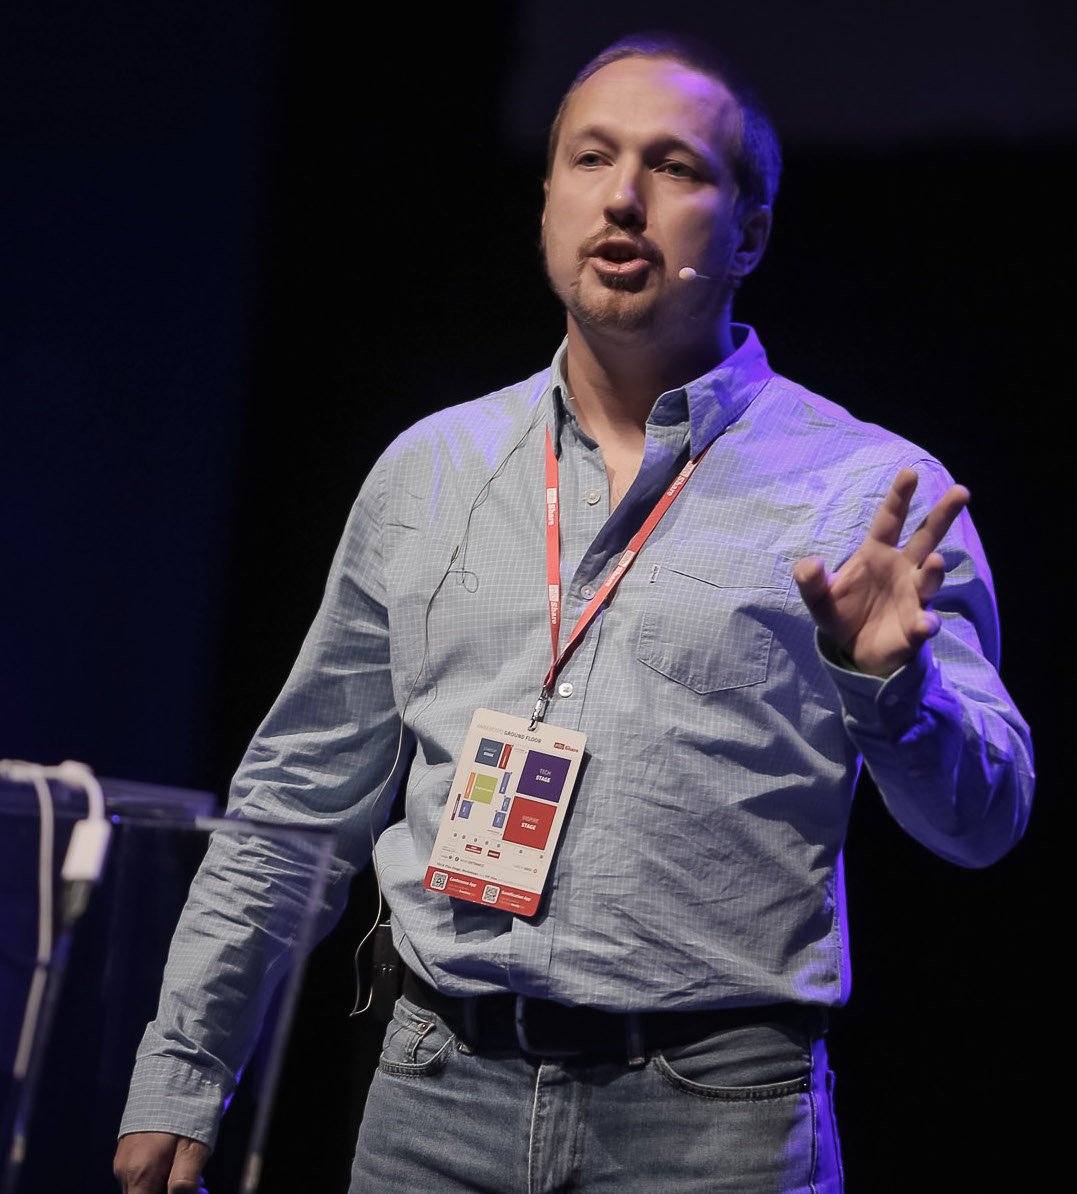
\includegraphics[height=3cm]{AntonPolyakov.jpg}
\end{tabbing}
}

%----------------------------------------------------------------------------------------
%	PERSONAL PROFILE
%----------------------------------------------------------------------------------------

\section{Personal Profile}
Practical tech lead with proven track of record delivering with teams of different sizes and spirit - from focused startup-like fast-paced groups to geo-distributed departments of 60+ engineers. Inspirer, speaker, executor, visioner and someone who strongly believes in leading by example.
My area of interests includes: streaming data processing, distributed systems, reactive system design, functional programming, in-memory processing.

%----------------------------------------------------------------------------------------
%	EDUCATION SECTION
%----------------------------------------------------------------------------------------

\section{Education}

\tabbedblock{
\bf{2008-2010} \> PhD, Math methods in economics - {Moscow Institute of Economics, Statistics and Informatics, Moscow} \\[5pt]
\>\+
\textit{PhD thesis - "FX Options streaming pricing model development"}
}

%------------------------------------------------

\tabbedblock{
\bf{2001-2007} \> MSc, Applied math and physics - \href{https://mipt.ru/english}{Moscow Institute of Physics and Technology, Moscow}\\[5pt]
\>Radio Engineering and Cybernetics \\
\>\+
\textit{MSc thesis - "Autonomous dsitributed multi agent systems"}
}

%----------------------------------------------------------------------------------------
%	EMPLOYMENT HISTORY SECTION
%----------------------------------------------------------------------------------------

\section{Employment History}

\job
{Sep 2015 -}{Present}
{Nordea Markets, Copenhagen, Denmark}
{http://www.nordea.com}
{Head of Application Development, Core Services and Risk, Capital Markets}
{Managing software development teams in Denmark and Poland (60+ developers in total) working on the key parts of the new Nordea Capital Markets IT ecosystem in Trading 
and Risk domain. Technical manager, solution architect and owner for number of critical systems and 
foundational components:
\begin{itemize}
\item{Core messaging layer and cloud-ready infrastructure (dynamic service discovery, containerized deployments, cluster based architecture facilitating canary rollouts, automatic failover and elastic scalability) for Capital Markets}
\item{Document-based Trade Vault serving trade contract information for Capital Markets system (multi
terabyte MongoDB-based solution)}
\item{New FRTB Market Risk infrastructure (> x10 capacity increase comparing to existing one,
reactive and on-demand computations comparing to overnight batch)}
\item{Improved Credit Risk system landscape to ensure continuous delivery model with vendor solution}
\end{itemize}

\rule{0mm}{5mm}\textbf{Technologies:} Java, Kafka, Redis, REST, Cassandra, MongoDB, Consul, Docker Swarm, Ansible}

%------------------------------------------------

\job
{Aug 2014 -}{Sep 2015}
{Nordea Markets, Copenhagen, Denmark}
{http://www.nordea.com}
{Head of Market Risk IT}
{Started as a crisis manager leading a team of 25 developers and business analysts.
Risk valuation engines were seriously below SLAs, suffered from substantial capacity, stability and scalability issues, required extensive manual support due to lack of automated deployment processes. Development process was nontransparent, ineffective and key-man dependent.
My goal was to bring systems back to SLA, (re) engineer  systems, bringing in
engineering culture, building strong development practice, ensuring agile and transparent development
processes.\\*
Achieved results:
\begin{itemize}
\item{identified the most problematic hot spot areas and developed an evolutionary strategy to stabilize and re-engineer critical
components. Following the strategy systems throughput and stability were substantially improved
in a smooth continuous way with neither business interruption nor massive regressions required}
\item{established transparent scrum-like process with strong ownership and ensured continuous delivery chain.
It required building the full continuous delivery pipeline and migrating existing legacy code base to
automatic deployment framework}
\item{cleaned up old systems and built a new microservice-based set of components leveraging web-scale
technologies like Redis and Kafka, employing reactive principles with RxJava and doing idempotent scalable
architecture achieving more than x100 times performance improvements in certain areas}
\item{established set of strong, mobile and self-organized engineering teams}
\end{itemize}
}

\job
{Mar 2012 -}{Jul 2014}
{Sberbank Technologies, Moscow, Russia}
{}
{Head of Risk IT development}
{Managed development and delivery of a global risk management platform (\$30+ mio budget, 30+ developers) for Sberbank.
\begin{itemize}
\item{Projects setup process including public tenders, high-level roadmap and budgeting}
\item{Setting up, communicating and owning department IT strategy to reach mid to long term business goals}
\item{Building and managing development teams in 3 regions (30+ devs, Russia and Belarus), setting up development process}
\item{Conceptual architecture and detailed architecture of critical components. Implemented SOA approach for
the platform, using reactive architecture (based on Akka), distributed computing and NoSQL concepts for solving non-trivial technical
challenges}
\end{itemize}
}

\job
{Sep 2007 -}{Mar 2012}
{Deutsche Bank, Moscow, Russia}
{https://autobahn.db.com}
{Assistant Vice President, abFX Options lead}
{Autobahn is Deutsche Bank's client-facing electronic trading platform delivering real-time trade execution, market analysis, order management and other advanced features. 
I was leading FX Options part of the platform. abFX Options is a low-latency geo-distributed service operating in 24x7 having points of presence in NY, London, Hong-Kong and Singapore. 
Major achievements: \\*
\begin{itemize}
\item{Designed, build and launched Deutsche's first FIX API for trading Options by leveraging abFX service backend capabilities}
\item{Launched first in class Options order execution platform (ATOM) capable of automatic real-time order fulfillment}
\item{Leveraging abFX server capabilities, successfully launched global RFQ engine for voice trading with possibilities to price arbitrarily complex products and doing post-trade/quote hit/miss analytics}
\end{itemize}
}

\job
{May 2005 -}{Nov 2006}
{Competentum Group, Moscow, Russia}
{https://competentum.com}
{Senior Java developer}
{Designing, coding and launching e-learning solutions for major American educational companies}

\job
{May 2004 -}{May 2005}
{Netcracker, Moscow, Russia}
{http://www.netcracker.comm}
{Java developer}
{Working on backend services for Netcracker OSS software. Java, Weblogic, JSP}

%----------------------------------------------------------------------------------------
%	IT/COMPUTING SKILLS SECTION
%----------------------------------------------------------------------------------------

\section{Software Engineering Skills}

\skillgroup{Programming Languages}
{
\textit{Java} - primary \\
\textit{Go, C} - no production experience\\
}

%------------------------------------------------

\skillgroup{Databases, tools and frameworks}
{
\textit{SQL (Oracle), MongoDB, Cassandra, Redis, ActivePivot}\\
\textit{Spring ecosystem (Cores, MVC, Data), Netflix OSS (Ribbon, Feign)}\\
\textit{Docker, Consul, Registrator, Swarm} - Docker ecosystem\\
\textit{Kafka, RabbitMQ, ZeroMQ} - messaging\\
}


%----------------------------------------------------------------------------------------
%	INTERESTS SECTION
%----------------------------------------------------------------------------------------

\section{Interests}

\interestsgroup{
\interest{Djudo, BJJ, MMA}
\interest{Distributed systems and streaming architectures}
\interest{Heavy metal guitar (playing in a band)}
\interest{Offroad}
\interest{Fishing}
}

%----------------------------------------------------------------------------------------
%	REFEREE SECTION
%----------------------------------------------------------------------------------------

\section{Referees}

\parbox{0.5\textwidth}{ % First block
\begin{tabbing}
\hspace{2.75cm} \= \hspace{4cm} \= \kill % Spacing within the block
{\bf Name} \> Matthew Bridgwater \\ % Referee name
{\bf Company} \> Nordea \\ % Referee company
{\bf Position} \> Global Head of Market Risk \\ % Referee job title 
{\bf Contact} \> \href{mailto:matthew.bridgwater@nordea.com}{matthew.bridgwater@nordea.com} % Referee contact information
\end{tabbing}}
\hfill % Horizontal space between the two blocks
\parbox{0.5\textwidth}{ % Second block
\begin{tabbing}
\hspace{2.75cm} \= \hspace{4cm} \= \kill % Spacing within the block
{\bf Name} \> Craig Dunham\\ % Referee name
{\bf Company} \> Nordea \\ % Referee company
{\bf Position} \> Chief Enterprise Architect \\ % Referee job title 
{\bf Contact} \> \href{mailto:craig.dunham@nordea.com}{craig.dunham@nordea.com} % Referee contact information
\end{tabbing}}

%----------------------------------------------------------------------------------------

\end{document}
